We developed a Lucene-based%
\footnote{\texttt{http://lucene.apache.org/}%
} IR system with the possibility of using diverse generic IR models: TF-IDF, BM25, Language Models (Dirichlet smoothing, and Jelinek-Mercer smoothing) as our baseline system. We achieved the best baseline effectiveness querying with the Description section of the patent application as it is also mentioned in \cite{xue2009transforming}, and using LM and BM25 scoring functions. We call this initial query: {\em patent query}. We conducted our experiments on CLEF-IP%
\footnote{\texttt{\url{http://www.ifs.tuwien.ac.at/~clef-ip/}}}% 
 2010 data collection, with 2.6 million European patent documents and 1303 English topics (queries). On the collection side, we only indexed English subset of each section of a patent (title, abstract, claims, and description), and IPC\footnote{International Patent Classification}% 
  code in a separate field. We also used the patent classification assigned to the query topics to filter search results to match at least one of the query IPC codes, as recommended in \cite{lopez2010patatras}. Our experiments showed that using IPC filter is itself a source of error because about 19\% of relevant patents in CLEF-IP 2010 data collection do not share any classification code with their query. However, for our analysis, we kept the filter on since it made the matching process between the query and documents notably faster. To evaluate the results, we used Mean Average Precision (MAP) and Average Recall.
 %\footnote{\texttt{For an accurate term analysis, we pruned out the source of errors related to data curation such as non-English patents, and IPC filter.}%
%}.
%\begin{figure*}
%\begin{center}
%\noindent\begin{minipage}[b]{0.3\linewidth}
%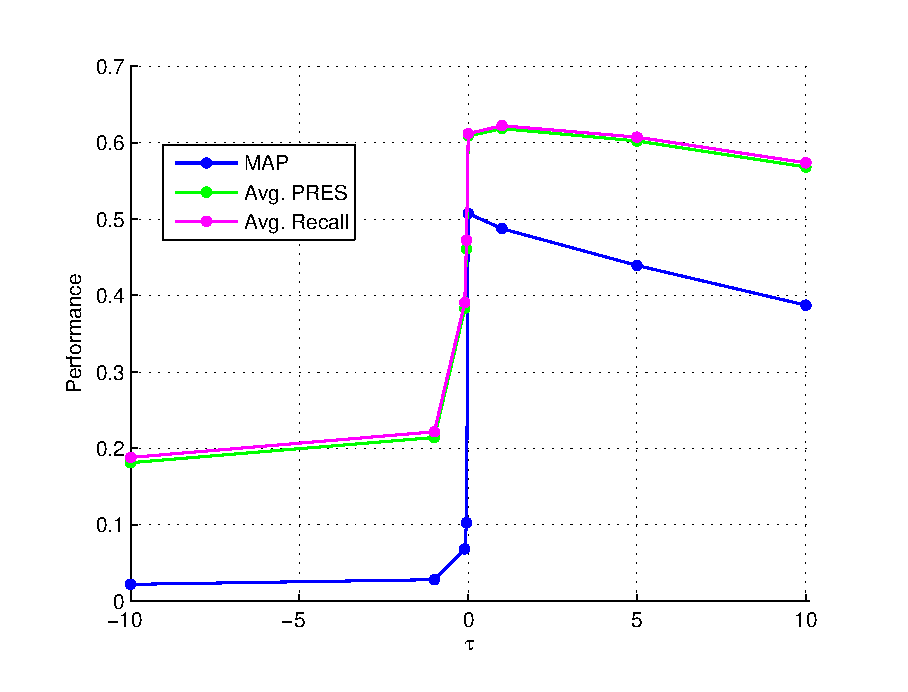
\includegraphics[width=\linewidth]{figs/extended-optquery-tau.eps}
%\end{minipage}%
%\hfill
%%\hspace{7mm}
%\begin{minipage}[b]{0.3\linewidth}
%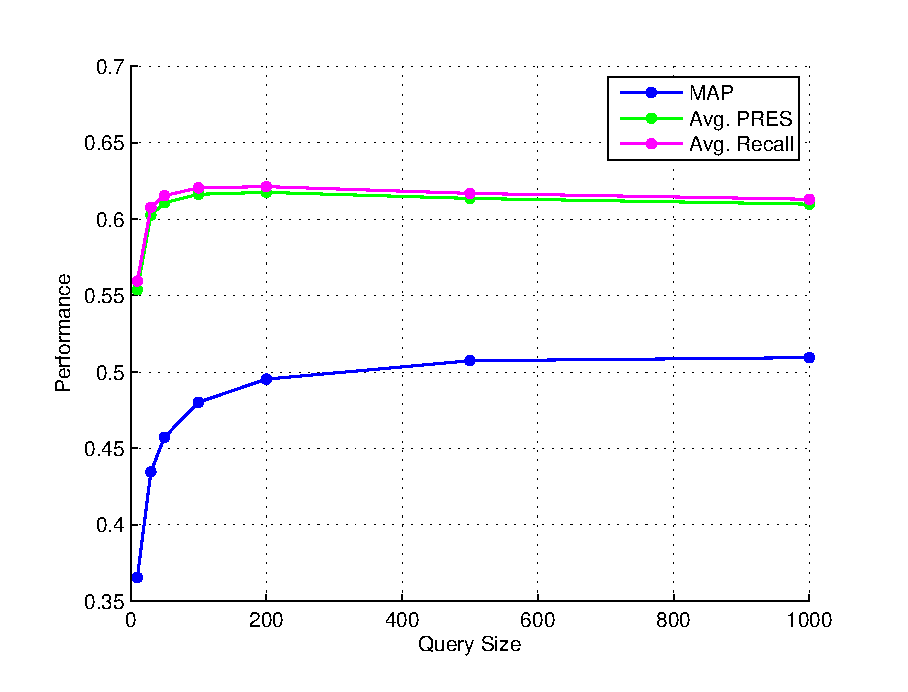
\includegraphics[width=\linewidth]{figs/opt-query-qsize.eps}
%\end{minipage}
%%\vspace{-3mm}\\
%%(a) \hspace{30mm}(b)\\
%\hfill
%%\hspace{7mm}
%\begin{minipage}[b]{0.3\linewidth}
%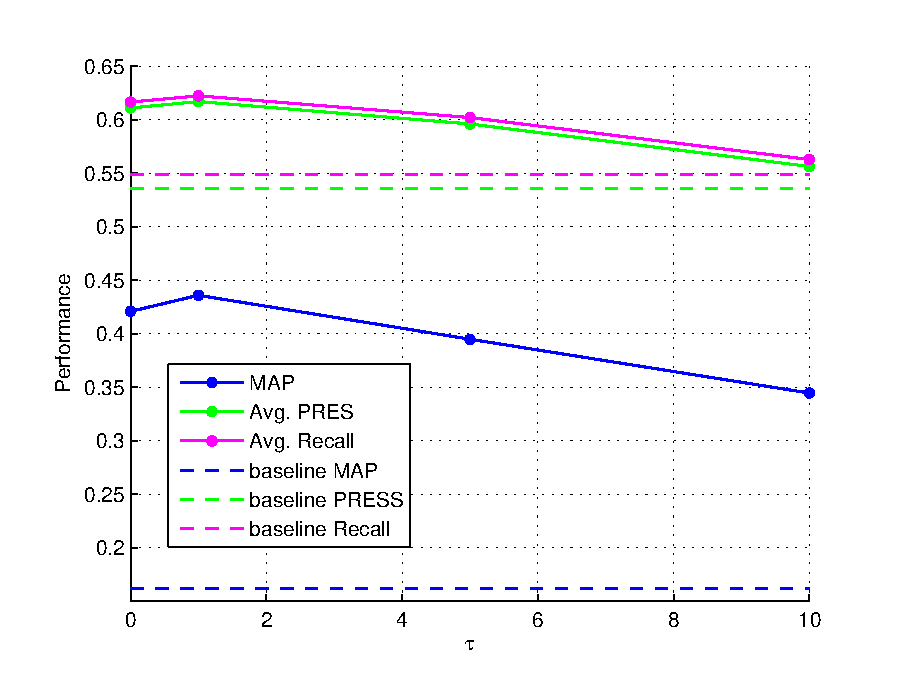
\includegraphics[width=\linewidth]{figs/opt-patentquery-tau.eps}
%\end{minipage}
%\vspace{-0.5mm}\\
% \hspace{2mm}(a) \hspace{55mm}(b) \hspace{58mm} (c)
%\caption{\footnotesize
%How score threshold($\tau$) and query size controls the performance.
%(a) Performance versus the score threshold. (b) Performance versus the query size. (c) System performance when we reduced the query by RF: $ query = Q\cap (useful \; terms) $, where $ Q $ is the patent query and $ useful\; terms = \{t| score_{RF}(t)>\tau\} $.}
%\vspace{-4mm}
%\end{center}
%\label{fig:control}
%\end{figure*}